\chapter{自动加样系统硬件设计方案的确定}
自动加样控制系统包括一个控制器,有若干个功能模块。控制器为$AT89C52$单片机,功能模块为直角坐标系中三个方向的步进电机运动模块、三个位置传感器模块、加样机构的液位传感器模块和步进电机驱动模块、清洗模块等。三个步进电机运动模块在驱动模块的作用下实现了在三维空间内任意位置的定位,位置传感器使得检测机械臂复位情况以及防止机械臂在运动过程中发生干涉,液位传感器检测加样机构到达液面以下的位置
\section{控制器的选型}
本研究选用的控制器为$AT89C52$单片机,它是一款8位$CMOS$单片机,由美国公司$ATMEL$推出。$AT89C52$单片机嵌有$8K bytes$可反复擦写的闪存$ROM$存储器和$256$ $bytes$数据存储器;32个输入输出($I/O$)接口线,3个16位定时计数器,一个全双工串行通讯口,同时含有两个外中断口,共六个中断源;此外,片内配置振荡器和时钟电路。其空闲工作模式能保证$CPU$停止工作的同时其它模块如存储器、中断系统正常工作,掉电保护模式能及时保存$RAM$内容,使振荡器失去作用并其它部件工作直到接收到复位信号以保护系统\supercite{bib14}。$AT89C52$单片机强大的功能使其能够应用在较为复杂的控制系统中。该控制器的最小系统由复位电路和时钟电路组成,简单可靠。其电路图如\ref{fig:5-1}

\begin{figure}[htbp!]
	\centering
	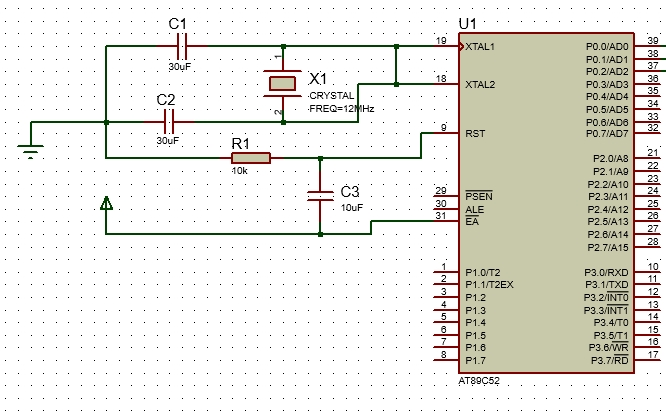
\includegraphics[height=7.5cm]{chap/figure/5-1.jpg}
	\caption{AT89C52最小系统简图}
	\label{fig:5-1}
\end{figure}

\section{步进电机驱动电路的设计}
一方面,$AT89C52$单片机的是输出功率非常小;另一方面,步进电机不能直接连接直流电源。因此,必须在步进电机和单片机之间接上驱动电路以保证前者的正常工作。步进电机的驱动器种类十分丰富,一般成熟步进电机产品都有配置的电机驱动器。在上一章节中我们选取了$Leetro$公司的DM5641E型号电机,那么步进电机的驱动器仍选取此公司配套的驱动器DMD605。该驱动器的脉冲响应频率最高可达360KHz,斩波频率为20KHz ,最大驱动电流达5.6A/相,其细分设定情况如表\ref{tab:5-1}。

\begin{table}[htbp]
	\centering
	\caption{DMD605细分设置}
	\begin{tabular}{cccccc}
		\toprule
		\toprule
		细分数  & 步数/转  &	SW5  & SW6  & SW7  & SW8 \\
		\midrule
		1  & 200  &  off  & off  & off  & off  \\
		2  & 400  & on  & on  & on  & on \\
		4  & 800  & on  & off & on  & on \\
		8  & 1600  & on  & off  & off  & on  \\
		\bottomrule
		\bottomrule
	\end{tabular}%
	\label{tab:5-1}%
\end{table}%


控制器$AT89C52$与DMD605驱动器的电路连线图如图\ref{fig:5-2}

\iffalse
\begin{table}[hfpb]
	\label{verilog}
	\caption{Verilog HDL语言能力总结}
	\hspace{0.5cm}
	\centering
	\begin{tabular} {p{40pt}p{50pt}p{170pt}p{130pt}}\toprule   
		\hei{描述级别} & \hei{抽象级别} & \hei{功能描述} & \hei{物理模型} \\ \midrule    
		& \song{系统级} & 用语言提供的高级结构能够实现所设计模块外部性能的模型 &        
		芯片、电路板和物理划分的子模块\\ \cmidrule{2-4}
		行为级& 算法级 & 用语言提供的高级功能能够实现算法运行的模型 &        
		部件之间的物理连接,电路板\\ \cmidrule{2-4}
		& RTL级 & 描述数据如何在寄存器之间流动和如何处理、控制这些数据流动的模型 &        
		芯片、宏单元\\ \midrule
		逻辑级 & 门级 & 描述逻辑门与逻辑门之间连接的模型     & 标准单元布图\\ \midrule
		电路级 & 开关级 & 描述器件中三极管和存储节点以及他们之间连接的模型 & 晶体管布图 \\ \bottomrule
	\end{tabular}
\end{table}
\fi






